\section{Trenutni pogled sveta na generativni AI}
Trenutna pozicija AI-a je vrlo diskutabilna. Do skorije, dosta kompanija poput NVIDIA i Microsofta su u potpunosti bili za korišćenje veštačke inteligencije u generativnom smislu. NVIDIA je čak napravila DLSS5 grafički alat koji u realnom vremenu utiče na samu grafiku video igara i koristi generativni AI kako bi dodali filtere na samu igricu. To utiče i na sam enterijer, eksterijer i anatomiju lica čoveka. Dosta gejmera i umetnika se pobunilo protiv ovog alata jer su neke likove promenili do te mere da više ne izgledaju prirodno. Takođe su se pobunili zato što potkopava umetničku slobodu, trud i rad dizajnera video igara. \cite{beregovyi2025visual}\\
CNN je na nacionalnoj televiziji objavio kako Microsoft i NVIDIA preispituju svoje odluke o korišćenju AI-a. Došlo je do tih mera da je Microsoft zabranio svojim radnicima prekomerno korišćenje AI-a, a NVIDIA je rekla da ih više košta da plate AI nego da imaju tim od pravih ljudi. \\

\begin{figure}[H]
        \centering
        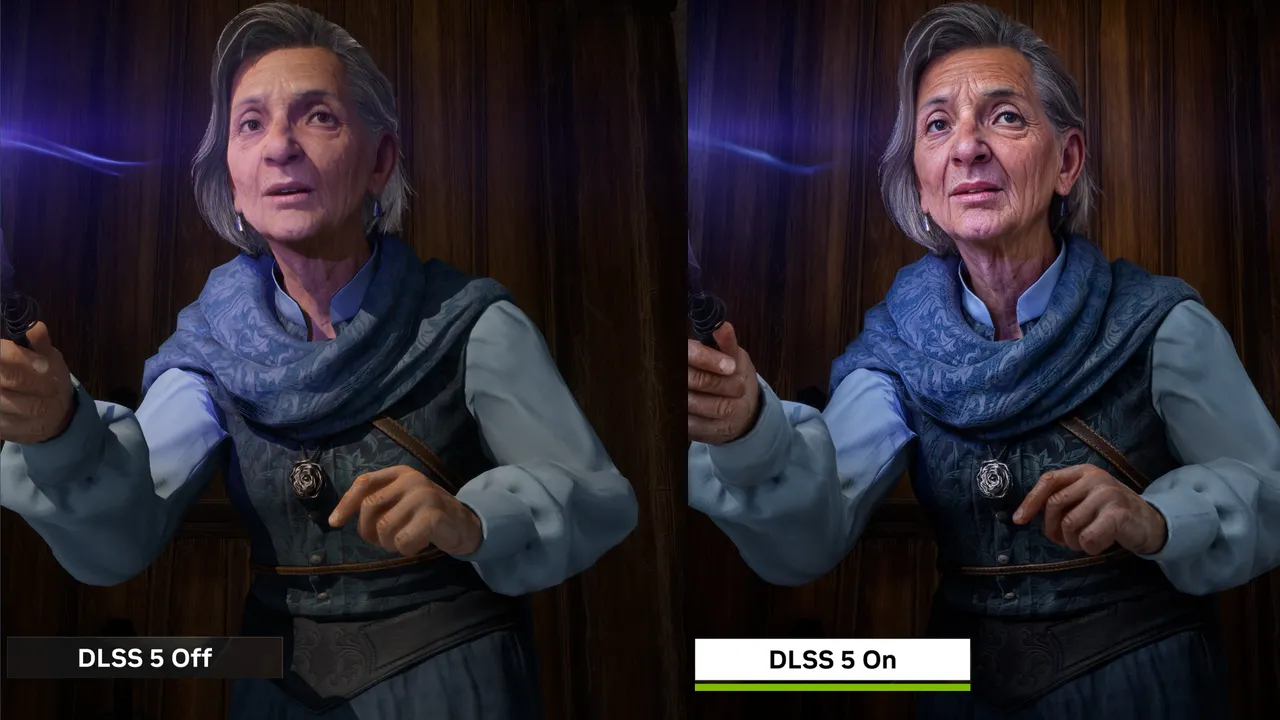
\includegraphics[width=0.6\linewidth]{Pictures/b4c3c9d1751d-nvidia-dlss-5-ai-slop-screenshot-comparison(1).png}
        \caption{Proces digitalizacije podataka}
    \end{figure}


\begin{wrapfigure}[17]{r}{0.5\textwidth}
    \centering
    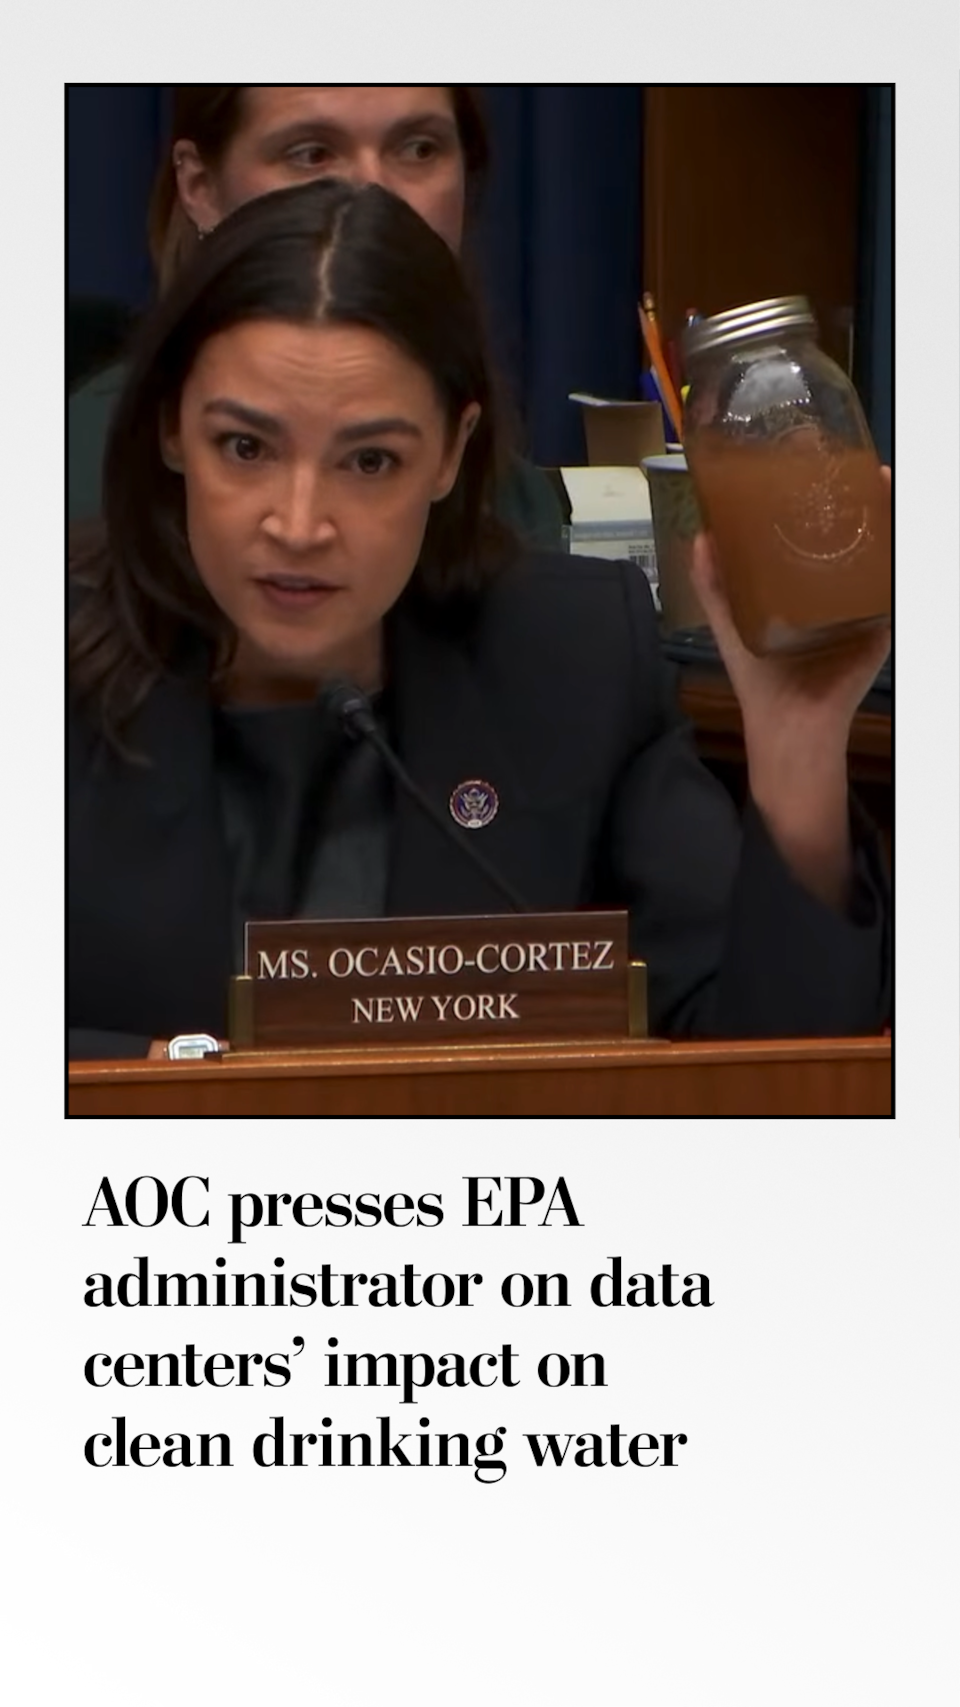
\includegraphics[width=0.3\textwidth]{Pictures/imrs.png}
\end{wrapfigure}

Papa Lav XIV je 15. maja 2026. godine potpisao svoju prvu Encikliku pod imenom ''Magnifica Humanitas'' u kojoj govori o tome da veštačka inteligencija treba služiti čovečanstvu. Enciklika se fokusira na to kako da očuva ljudsko dostojanstvo u eri veštačke inteligencije. Na televiziji je govorio o tome kako je veštačka inteligencija zlo protiv čovečanstva ukoliko se koristi u pogrešne svrhe. \\



Pored toga što generativni AI krade slobodu i originalnost samih umetnika bez razgovora sa njima, generativni AI proizilazi iz Data Centra koji uništavaju pijaću vodu. Velike korporacije prave Data Centre koje uništavaju nju do te mere da voda sa česme postaje braon i zagađena. Koriste toliko resursa da ljudi rapidno počinju da gube pristup normalnoj vodi i moraju da kupuju flaširanu vodu da bi je pili ili održali osnovnu higijenu.\cite{tangermann2025meta_water}

\section{Zaključak}

Razvoj generativne veštačke inteligencije je doneo velike promene u oblasti vizuelnih umetnosti, otvarajući vrata o ozbiljnim etičkim i pravnim pitanja. Kao što je prikazano, modeli veštačke inteligencije funkcionišu na osnovu velikih količina podataka. Često se uzimaju podaci o crtežima bez eksplicitne dozvole autora, čime se direktno dovodi u pitanje zaštita autorskih prava.

Alati poput Glaze i Nightshade predstavljaju prve konkretne korake ka zaštiti umetnika u digitalnom okruženju. Dok Glaze otežava imitaciju umetničkog stila, Nightshade aktivno utiče na ponašanje modela kroz trovanje podataka, a njihova kombinovana upotreba pruža složeniji i efikasniji vid odbrane. Ipak, ovi alati nisu konačno rešenje, jer njihova efikasnost zavisi od načina treniranja modela i budućih tehnoloških unapređenja. Kreatori ovih alata se iz dana u dan zalažu da ih naprave boljim i pogodnijim za korišćenje. Uvek će postojati momenti kada Glaze i Nightshade neće biti dovoljni. Stoga, cilj kreatora je da produže njihov trenutni rok trajanja koliko god je to moguće.

Pored tehničkih izazova, neophodno je sagledati i širi društveni kontekst. Debata o ulozi veštačke inteligencije pokazuje duboku podeljenost između tehnološkog napretka i očuvanja ljudske kreativnosti. Dovodi se u pitanje i ekološke posledice nastale od strane infrastruktura koje podržavaju AI sisteme.

U budućnosti će biti ključno pronaći balans između inovacije i regulacije. Zaštita umetnika se ne može osloniti isključivo na tehnička rešenja, već zahteva i pravni okvir, transparentnost u razvoju AI sistema i veću svest o vrednosti originalnog ljudskog stvaralaštva. Veštačka inteligencija treba da bude alat koji pruža pomoć čoveku, a ne da ga zameni i ograniči njegovu kreativnost.
